
\section{Introduction}
One of the most important ascpects of machine learning is classification. Typical algorithms and models
that are used for classification include logistic regression, naive bayes, decision trees and so on. In the early 90s, 
Vladimir Vapnik and his colleagues developed a new algorithm called \emph{Support Vector Machine (SVM)}, which is optimized for classification and regression analysis. In this paper,
we will focus on the main usages of SVM, including the generalization of linear decision boundaries for classification.
We will also discuss the role of kernel in SVM, as well as the implementation, evalution methods, application and many
different aspects of SVM.

In order to thoroughly understand the classification problem, we first need to look at a simple example in one dimension.
Suppose there are two groups of data points that are separately distributed on a one-dimension number line. The classification then
becomes obvious: The threshold that separates both groups simply lies in the middle of the the most outward data points
from both groups. This classification method is called the \emph{maximum margin classifier}, since the margin that separates both
groups is maximized.

\begin{figure}[h]%
    \begin{center}%
        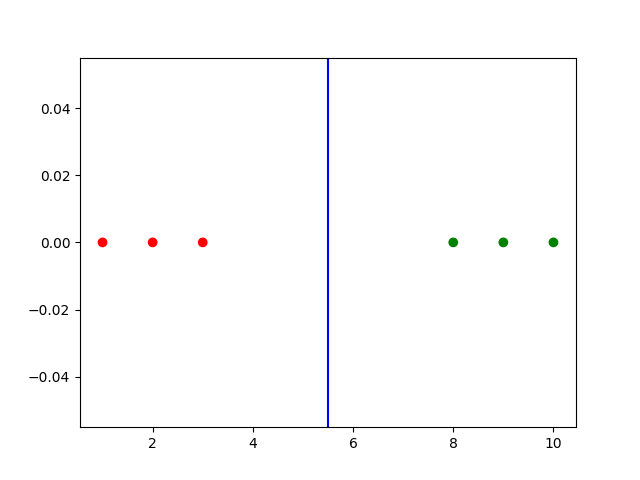
\includegraphics[scale=0.3]{Maximum_Margin_Classifer.png}%
        \caption{Maximum Margin Classfier}\label{fig:}%
    \end{center}%
\end{figure}

Nevertheless, the maximum margin classifier is not always applicable, since the data points are not always idealy distributed
in a separated way. If an outlier happens to appear in the dataset, it would push the threshold to one side, since the data point
is much closer to the other group. This would result in a severe misclassification, since the data that are close to one
group now belongs to the other group because of the shift of the threshold. A solution to this problem is to allow some
misclassification, so that the threshold has higher bias and is less sensitive to outliers and the classifier performs better
when there is new data. This margin that allows some misclassification is called the \emph{soft margin}. The determination of soft margin 
could be tricky, since there are limitless points of thresholds to choose from. One way to find the optimal threshold
is to use Cross Validation. Cross Validation is a method that splits the dataset into several parts. For each repetition, 
one part of the dataset is used for testing and the rest is used for training. After training through all the repetition, the 
average position of the threshold represents the most ideal position of the soft margin. This classifier is called
soft margin classifier, also known as support vector classifier. The name "Support Vector" derives from the fact that
the data points that are closest to the threshold are called support vectors.

\begin{figure}[h]%
    \begin{center}%
        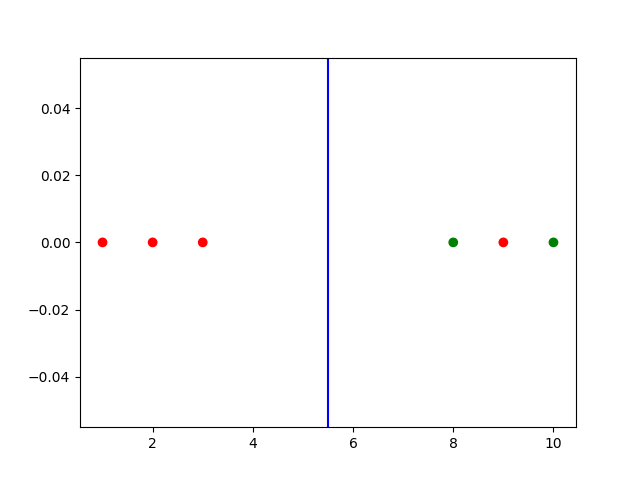
\includegraphics[scale=0.3]{Support_Vector_Classifier.png}%
        \caption{Support Vector Classfier}\label{fig:}%
    \end{center}%
\end{figure}

In reality, chances are that the data is not only one-dimensional. In fact, almost all of the data that we work with
is multi-dimensional. In order to represent the data in a multi-dimensional space, we need to use vectors. In this case,
the idea of hyperplane is introduced. A \emph{hyperplane} is a threshold that separates the data in a multi-dimensional space,
which is formally defined as a flat affine subspace.\cite{R9} The support vector classifier is able to deal with this case as well.
It finds the hyperplane that separates the data in a way that the margin is maximized. The exact algorithms and the
mathematical derivation will be discussed in the next section.

However, the support vector classifier is still not suitable for data that is not linearly separable, even though 
the support vector classifiers allows misclassifications and is less sensitive to outliers.
\begin{figure}[h]%
    \begin{center}%
        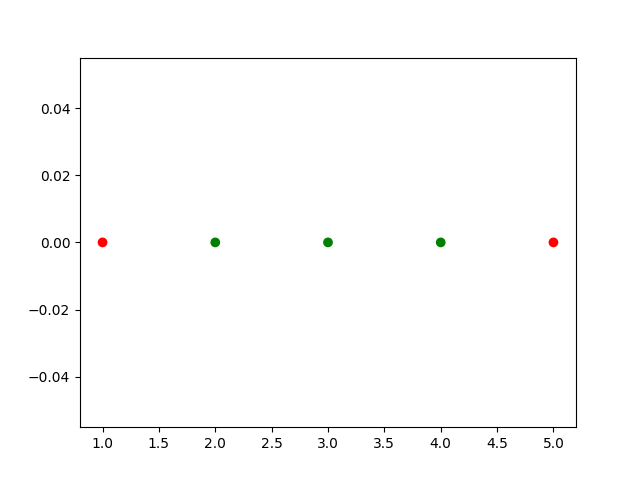
\includegraphics[scale=0.3]{Non_Linearly_Separable_Data.png}%
        \caption{Non Linearly Separable Data}\label{fig:}%
    \end{center}%
\end{figure}

Usually, we use a \emph{kernel} to deal 
with this case, which is a function that maps the data into a higher dimensional space, so that the data becomes linearly
separable. The SVM implements the idea of kernel without transforming the data into a higher dimensional space. This concept is 
called \emph{the kernel trick} and is a crucial part of SVM. This trick allows SVM to cast nonlinear variants to dot products,
enabling easier computation and better performance. \cite{Kernel2}
\begin{figure}[h]%
    \begin{center}%
        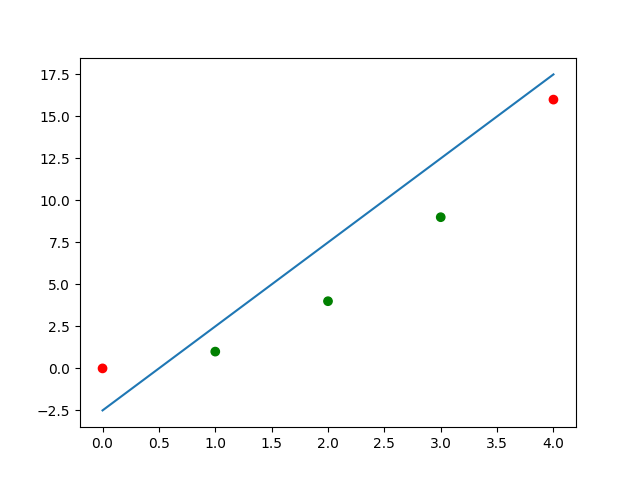
\includegraphics[scale=0.3]{Kernel_Separation.png}%
        \caption{Kernel Transformation}\label{fig:}%
    \end{center}%
\end{figure}
